
\chapter{Muscle Fibers and Motor Units}\label{sec:muscle_fibers_and_motor_units}
The activation of muscle fibers is governed by the functional organization of the fibers in motor units (MU). An MU is the set of fibers that are innervated by the same $\alpha$-motor neuron, together with the neuron. If a motor neuron fires, all muscle fibers within the MU are activated. The association of the muscle fibers with MUs needs to be specified for electrophysiology simulations that consider activated muscle fibers. This chapter describes algorithms to achieve an MU-fiber association based on biophysical principles.

\section{Introduction}\label{sec:mu_intro}
Given a number of muscle fibers, the goal is to assign each fiber to one MU out of a set of given MUs. A muscle with a fusiform geometry, such as the biceps brachii is considered. Because muscle fibers do not branch or interrupt within the belly of such a muscle, the task can be reduced to the 2D problem on a cross section of the muscle.

Properties of MUs have been subject to various investigations in literature. The number of MUs in a human muscle can be estimated by anatomical and physiological methods \cite{MacIntosh2006}. Anatomical methods include counting large-diameter fibers in post mortem tissue. The morphologic studies of \cite{Feinstein1955} revealed high variations between different muscles. For example, the brachioradialis muscle has an estimated number of \num{333} MUs with \num{410} muscle fibers on average whereas the external rectus muscles in the eye have \num{2970} MUs with an average of only 9 muscle fibers. 

Physiological methods involve comparing the electrical and mechanical responses of artificially activated muscles, e.g., as in \cite{Milner-Brown1973b,Thomas1990b}. Typically, a high number of MUs with a smaller force or electric response is observed and a smaller number of MUs with a higher response. 
The review of \cite{Enoka2001} collects available experimental results and concludes an exponential distribution of the number of fibers per MU over all the MUs in a muscle.
% Enoka and Fuglevand (2001): Motor unit physiology: some unresolved issues

The spatial arrangement of the fibers of an MU can be revealed by a histochemical method \cite{brandstater1969histochemical}. It was found that the fibers of an MU appear at random positions but are grouped in a sub region of the muscular cross section. The size of the sub region varies among muscles and fiber types and can be as large as one quarter of the cross section, as in the tibialis anterior of the rat \cite{Edstrom1968}. Although the fibers of an MU are located in proximity they usually do not touch each other, i.e., there are always fibers of other MUs in between the fibers associated with an MU.

In our algorithm for assigning fibers to MUs we incorporate the following properties that are founded on biophysical experiments. 
\begin{itemize}
\item[(a)] The number of fibers per MU is  exponentially distributed. 
\item[(b)] The fibers of an MU are spatially distributed around a center point of the MU territory.
\item[(c)] The MU center points are reasonably separated from each other. However, the MU territories intermingle. 
\item[(d)] The spatial extents of the MU territories are proportional to the number of fibers of the MUs. 
\item[(e)] The exact locations of the fibers are random, but the overall density of fibers in the muscle is approximately constant. 
\item[(f)] Neighboring fibers are not innervated by the same motor neuron and therefore belong to different MUs.
\end{itemize}

Further physiological properties of fibers such as their fast or slow-twitch type as well as the distribution of electrical and mechanical properties are not subject to the fiber assignment algorithm. They are considered during configuration of the simulations of electrophysiology or muscular contraction.

\subsection{Related Works}
Simulations involving individually resolved muscle fibers are scarce in the literature. Therefore, not much previous work exists regarding methods to algorithmically assign fibers to MUs. The chemo-electro-mechanical skeletal muscle framework of \cite{Heidlauf2013} uses a method introduced in \cite{Roehrle2012} where center points of MU territories are positioned normally distributed around two distinct weighting centers for fast- and slow-twitch fibers. 
The algorithm randomly selects from certain sets of fibers and assigns them to MUs with exponentially increasing MU sizes. 
The method is applied to determine up to 50 MUs in the tibialis anterior (TA) muscle.

This algorithm fulfills the previously formulated properties (a)-(e). Among those, the fulfillment of (c) is not guaranteed but may be given by the random nature of the algorithm. An assumed issue regarding property (b) is that no predictions can be made about the fiber locations of the larger MUs. The larger MUs get assigned to previously unassigned fibers in a late stage of the algorithm, after most of the fibers have been selected for smaller MUs. The largest MU simply gets associated with all remaining fibers that were not selected for other MUs. In the worst case, these fibers can accumulate at multiple different regions, e.g., at boundaries of the muscle which is not physiological.

Instead of the 3D setting in \cite{Roehrle2012} that was needed for the complex anatomy of the TA muscle, we restrict our problem to a 2D cross section of a fusiform muscle such as the biceps brachii. In comparison, our method creates MU territories of equal quality for all MUs and additionally fulfills property (e). Slow- and fast-twitch fibers are not treated differently by our algorithm, their properties are considered later in the simulation settings.

3D Simulations of skeletal muscle exist that treat MU association as homogenized property in the muscle volume. The approach in \cite{harry2018} assigns volume fractions of MUs to every spatial point of a 3D FEM discretization grid. MU center points are selected randomly ensuring a minimal distance. Prescribed volume fractions are sequentially assigned for each MU. The degree of intermingling can be adjusted by a parameter. It is shown that the algorithm highly depends on the order in which the MUs are traversed. The algorithm fulfills the properties (b)-(e), fulfilling (a) is possible by using appropriate parameter values.

In comparison, our method is targeted at MU assignment to individual fibers. However, distributing volume fractions is also the first step in our method. The volume fractions are interpreted as probabilities of the fibers being assigned to the respective MU. Therefore, our method can also be used as generator for homogenized formulations. A difference is that our method does not depend on a traversing order of MUs and ensures the exponential distribution of MU sizes.

\subsection{Two Alternative Premises for Motor Unit Assignment}
% Röhrle2012: TA 12 elements, MU association
% Heidlauf2013: 400 fibers, TA, OpenCMISS, mechanics

We identify two different sets of requirements which lead to two different methods.
Both methods fulfill the properties (a)-(f) listed in \cref{sec:mu_intro}.
The first premise is to assign motor units to a given number of fibers such that every fiber is associated with one MU. The second, alternative premise is to assign motor units only to a portion of the given set of fibers, discarding unassigned ones and thereby reducing the resulting set of fibers.

With the first setup, simulations of muscles that are gradually activated by motor neurons are possible. Activating the full muscle corresponds to activating all MUs and, in consequence, all muscle fibers. In reality, it is hardly possible to voluntarily activate all fibers in a muscle. This approach is also chosen in the presented literature, \cite{Roehrle2012} and \cite{harry2018}.

The second setup corresponds to modeling only a part of the muscle. The discarded fibers can be seen as belonging to other MUs that are not part of the simulation. When running highly parallelized simulations containing a large number of fibers, the missing fibers can introduce load imbalances, if they are computationally treated equally to the fibers with MUs. Even if no extra computational time is spent for the discarded fibers, a parallel domain decomposition becomes more involved than with the first setup where all fibers in a grid are present.

An advantage of the second setup is that the MU assignment to the fibers is generally easier. It also has its analog in volume fraction methods, where scalar fields of factors $f_k: \Omega \subset \R^3 \to [0,1]$ representing multiple MU territories, $k=1, \dots, n_\text{MU}$, can be easily defined. With this setup it is possible, for example, to perform analogous EMG simulations with the Multidomain model of \cite{Klotz2020} and the fiber based model of \cite{Mordhorst2015}.

In the remainder of this chapter, \cref{sec:method1_assignment} presents method 1, which fulfills the first premise where all fibers are associated to the MUs. Next, \cref{sec:method2_selection} introduces method 2, which only associates some fibers to MUs. Methods 1 and 2 fulfill the properties (a)-(e). Two derived methods 1a and 2a are subsequently constructed in order to also fulfill property (f). They are presented in \cref{sec:method3_modification}. Results and a discussion is given in \cref{sec:mu_results_and_discussion} before the chapter ends with a conclusion in \cref{sec:mu_conclusion}.

\section{Method 1: Assignment of Motor Units to a Given Set of Fibers}\label{sec:method1_assignment}

In our methods to assign MUs to muscle fibers, the considered set of muscle fibers is organized in a regular grid. \Cref{fig:mu_grid0} shows 
a part of the cross section of a skeletal muscle, the domains of individual fibers are visible. \Cref{fig:mu_grid1} visualizes the representation of muscle fibers in our simulations. In this figure, a relatively low number of 49 fibers was modeled. The fibers are approximated by 1D lines with uniform spacing in radial direction. For the algorithms to assign MUs to fibers, the muscle cross section is considered as a logical 2D grid with a quadratic number of $n \times n$ fibers. Such a grid is visualized in \cref{fig:mu_grid2}.

\begin{figure}%
  \centering%
  \begin{subfigure}[t]{0.32\textwidth}%
    \centering%
    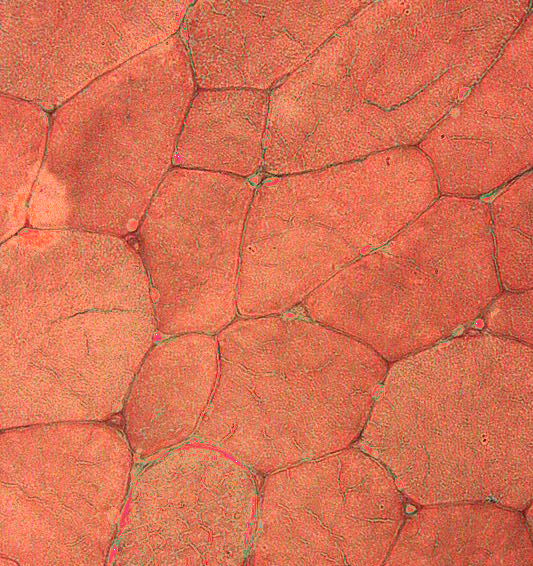
\includegraphics[width=\textwidth]{images/motor_unit_assignment/mus1.png}%
    \caption{Muscle fibers in the cross section of a muscle visualized by Gömöri trichrome stain\footnotemark}%
    \label{fig:mu_grid0}%
  \end{subfigure}
  \quad
  \begin{subfigure}[t]{0.28\textwidth}%
    \centering%
    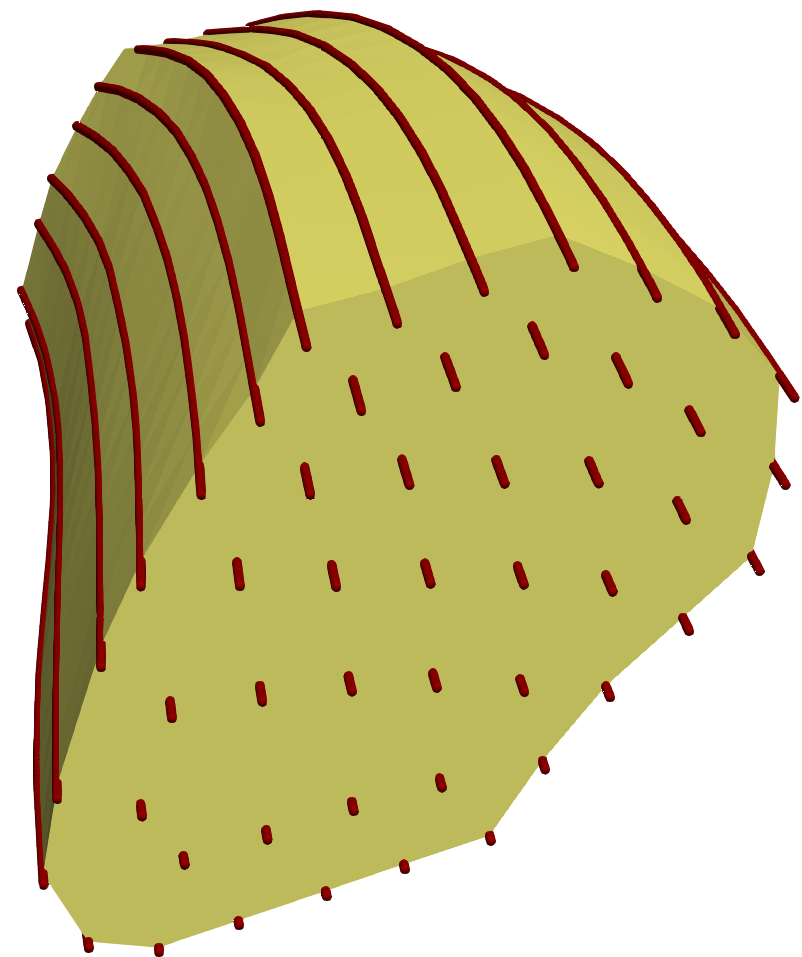
\includegraphics[width=\textwidth]{images/motor_unit_assignment/muscle_mesh_fibers.png}%
    \caption{A cut open muscle with $49$ muscle fibers in the simulation domain}%
    \label{fig:mu_grid1}%
  \end{subfigure}
  \quad
  \begin{subfigure}[t]{0.33\textwidth}%
    \centering%
    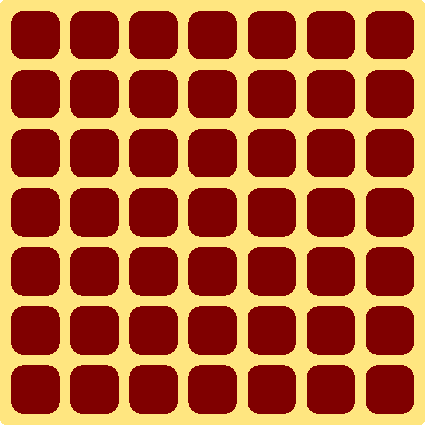
\includegraphics[width=\textwidth]{images/motor_unit_assignment/muscle_fibers_grid.pdf}%
    \caption{A quadratic grid of $7 \times 7$ fibers, used for the methods to assign MUs to fibers.}%
    \label{fig:mu_grid2}%
  \end{subfigure}
  \caption{Representation of muscle fibers for the methods to associate fibers with MUs: From the real muscle to a quadratic grid.}%
  \label{fig:mu_grid}%
\end{figure}%

\footnotetext{Image copyright © 25/12/2010 Michael Bonert (\url{https://commons.wikimedia.org/wiki/User:Nephron}), CC BY-SA 3.0 (\url{https://creativecommons.org/licenses/by-sa/3.0/legalcode}). The picture shows mitochondrial myopathy, it was cropped and the color was adjusted to make the \say{ragged red fibers} less prominent.}
\stepcounter{footnote}


The first method for the assignment of MUs to a given set of fibers associates the $n \times n$ fibers to a set of $n_\text{MU}$ motor units.
First, for each fiber ${(i,j)}$ in the grid, the probabilities $p(i,j,k_\text{MU})$ to be assigned to MU $k_\text{MU}$ are computed. This computation involves the solution of an optimization problem. Second, the sampling step assigns the actual MU indices to the fibers.

\subsection{Stochastic Formulation of Motor Unit Assignment}\label{sec:stochastic_formulation_and_algorithm}

In order to fulfill the formulated properties, the following three conditions are enforced on the probabilities. 
\begin{itemize}
\item[(i)] The probabilities at every fiber  have to be valid, i.e., positive and sum up to 1 for all MUs.
\item[(ii)] The portions fibers associated to MUs have to approximately follow an exponential progression $q$, with MU 1 containing the least and MU $n_\text{MU}$ containing the most fibers.
\item[(iii)] For any given MU, the spatial arrangement of its fibers in the cross sectional plane is described by a radial kernel function $\hat{p}$. The fiber density of the MU increases when moving closer to the center point of the MU. This condition approximates the fact that the fibers of an MU are located in proximity, forming the MU territory.
\end{itemize}

The exponential progression $q$ in condition (ii) is defined as follows,
%
\begin{align}\label{eq:mus_q}
  q(k_\text{MU}) = b^{k_\text{MU}} / \s{\ell=1}{n_\text{MU}} b^\ell.
\end{align}
%
% f(x) = 1/(1+a*x^2),  ∫f(x)dx = arctan(sqrt(x)*x)/sqrt(a) + c
% stddev = sqrt(variance) = sqrt(∫{-∞,+∞} (f(x)-0)^2 dx) = sqrt(pi/(2*sqrt(a)))
% => a = pi^2 / (4*\sigma^4)
%
% 
The basis $b$ is a parameter and should be set to a value greater than one, e.g., $b=\num{1.2}$. \Cite{Enoka2001} formulate the function to be proportional to $\exp(\log(R)/n_\text{MU}\cdot k_\text{MU})$ where $R$ is the constant ratio between the sizes of the largest and smallest MUs. Our form is equivalent with $b = R^{1/n_\text{MU}}$.

The value of $q$ in \cref{eq:mus_q} is always positive. The division by the scaling factor ensures that the probabilities for all MUs sum up to one. Thus, condition (i) is fulfilled. The construction with the exponential function fulfills condition (ii).

For condition (iii), center positions $\bfx_{k_\text{MU}}, k_\text{MU}=1, \dots, n_\text{MU}$ of the MU territories are defined. 
The center positions are quasi-randomly selected inside the inner 80\% of the $n \times n$ grid of fibers. A band at the boundary with width of 10\% is not considered because the MU center points should not be at the border of any MU territory but rather at their center.

The used quasi-random sequence is the following Weyl low-discrepancy sequence \cite{Weyl1916}:
\begin{equation}\label{eq:weyl}
  \begin{array}{lll}
    x_0 = 0.5, \qquad &y_0 = 0.5,\\[4mm]
    x_{i} = x_0+(i\cdot \alpha_1) \mod \num{1.0}, \qquad\qquad 
    &y_{i} = y_0+(i\cdot \alpha_2) \mod \num{1.0},\\[4mm]
    \text{with }\alpha_1 = \num{0.5545497}, \qquad &\alpha_2 = \num{0.308517}.
  \end{array}
\end{equation}
It is known that the sequences $x_i$ and $y_i$ are equidistributed in $[0,1)$ for any irrational $\alpha_1$ and $\alpha_2$ \cite{Weyl1916}. The chosen values lead to a sequence of 2D points $(x,y)\in $$[0,1)^2$ with low discrepancy and a good coverage of the domain for any number of sequence elements. Accordingly, the MU territory center points are defined as 
%
\begin{align*}
  \bfx_{k_\text{MU}} = \big((0.1 + 0.8\,x_{k_\text{MU}})\,n,\, (0.1 + 0.8\,y_{k_\text{MU}})\,n\big)^\top
\end{align*}
%
The radial kernel function $\hat{p}$ that describes the spatial probability distribution for a given MU $k_\text{MU}$ according to condition (iii) is defined as follows,
\begin{align}\label{eq:phat_kernel}
  \hat{p}(i,j,k_\text{MU}) = \dfrac{1}{1 + a\,\vert\bfx_{k_\text{MU}} - \bfx_{i,j}\vert^2}, \quad \text{with }a = \dfrac{\pi^2}{4\sigma^4}.
\end{align}
The coordinates $i$ and $j$ specify the grid point $\bfx_{i,j} = (i,j)^\top$ of the fiber. The factor $a$ is computed from the given standard deviation $\sigma$ of the spatial distribution of the MU territory around the center point. A lower value of $\sigma$ leads to smaller and \say{sharper} MU territories, for higher values of $\sigma$, the MU territories intermingle more with each other.
\Cref{fig:mu_phat} shows the graph of the function for $\sigma=1$. 

This kernel function was chosen because it can be computed efficiently with a low number of basic operations unlike, e.g., a Gaussian kernel function which requires costly evaluation of an exponential function.

\begin{figure}%
  \centering%
  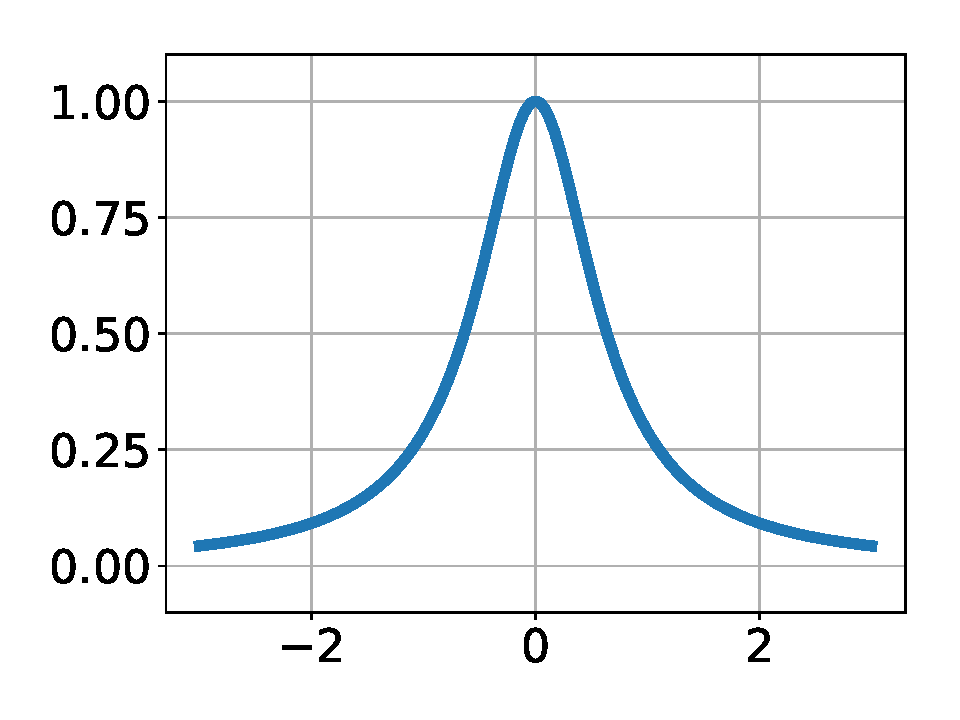
\includegraphics[width=0.4\textwidth]{images/motor_unit_assignment/phat.pdf}%
  \caption{Function $1/(1+a\,|x|^2)$, similar to $\hat{p}$ of \cref{eq:phat_kernel}, for $\sigma=1$.}%
  \label{fig:mu_phat}%
\end{figure}


If the kernel function $\hat{p}$ in \cref{eq:phat_kernel} is used to describe the probability of fiber $(i,j)$ to be in MU $k_\text{MU}$, then condition (iii) is fulfilled but conditions (i) and (ii) will not automatically be fulfilled. Instead of $\hat{p}$, a derived term $p(i,j,k_\text{MU})$ is introduced in the following that satisfies all requirements.

To ensure condition (ii), additional scalar factors $\lambda_k, k=1\dots n_\text{MU}$ for the MUs are introduced that yield the required exponential distribution.
To ensure condition (i), the term is normalized by a respective division. The resulting formulation is given as follows:
\begin{align}\label{eq:mu_p}
  p(i,j,k_\text{MU};\{\lambda_k\}_{1\dots n_\text{MU}}) = \dfrac{\hat{p}(i,j,k_\text{MU}) \cdot \lambda_{k_\text{MU}}}{\s{\ell_\text{MU}=1}{n_\text{MU}} \hat{p}(i,j,\ell_\text{MU}) \cdot \lambda_{\ell_\text{MU}}}.
\end{align}

Now, the factors $\{\lambda_k\}_{1\dots n_\text{MU}}$ have to be determined accordingly. Setting $\lambda_{k_\text{MU}} = q(k_\text{MU})$ would not yield the required exponential distribution of probabilities, because the MU center points $\bfx_{k_\text{MU}}$ have varying distances between each other.
Therefore, the accumulated total probability of all fibers to be associated to a particular MU is different for each MU. This is the case even before scaling with any factors $\{\lambda_k\}$.

Instead, the values of the factors have to be determined by solving a global optimization problem.
The objective function to be minimized is given by%
\begin{align}\label{eq:mus_objective}
  F(\{\lambda_k\}_{1\dots n_\text{MU}}) = \s{k_\text{MU}=1}{n_\text{MU}} \left(q(k_\text{MU}) - \s{i=1}{n}\s{j=1}{n}p(i,j,k_\text{MU};\{\lambda_k\}_{1\dots n_\text{MU}}) / n^2\right)^2.
\end{align}
It sums up the quadratic error for every MU between the desired, exponentially distributed probability $q(k_\text{MU})$ per fiber and the achieved probability per fiber under the current set of the scaling factors $\lambda_k$. 
The achieved probability is computed by a sum over all fibers $(i,j)$ and the formulated radial probability density function $p$ divided by $n^2$ to get the value per fiber.
After solving the optimization problem and plugging the factors $\{\lambda_k\}$ into \cref{eq:mu_p} we get every probability for a fiber to be in an MU by \cref{eq:mu_p}. The optimization problem is described in more detail in the following section.

\subsection{Algorithm to Solve the Optimization Problem}
The optimization problem to be solved in order to compute the scaling factors in \cref{eq:mu_p} can be stated as:
\begin{align}\label{eq:mus_opt}
  \text{``Find}\quad \{\lambda_k\}_{1\dots n_\text{MU}} \text{ with } \lambda_k > 0 \quad \text{ s.t. } \quad F(\{\lambda_k\}_{1\dots n_\text{MU}}) \quad \text{ is minimal''.}
\end{align}
The objective function $F$ was given in \cref{eq:mus_objective}. The solution is obtained by a Quasi-Newton method, more specifically the limited-memory version of the \emph{Broyden}-\emph{Fletcher}-\emph{Goldfarb}-\emph{Shanno} algorithm with box constraints by the authors of \cite{byrd1995limited}. Their Fortran implementation is made accessible in Python by the \emph{SciPy Optimize} package.

With increasing number $n^2$ of fibers and increasing number $n_\text{MU}$ of MUs, the evaluation duration for the objective function and the number of optimization parameters increases. For numbers about $n^2 > 1000$ and $n_\text{MU} > 25$, the solution times become unfeasible.

As a remedy we develop an algorithm to split the large optimization problem into multiple smaller ones which reduces the total runtime. 
The set of factors $\{\lambda_k\}_{1\dots n_\text{MU}}$ is partitioned into chunks, i.e., subsets of given size $n_\text{per\_chunk}$ leading to a total of $n_\text{chunks} = \lceil n_\text{MU} / n_\text{per\_chunk} \rceil$ chunks.
Remainder chunks towards the end potentially get one set element less. 
The factors for chunk number $c$ are selected in a strided manner as $\{\lambda_k\}$ with indices ${k=c, c+n_\text{chunks}, c+2\,n_\text{chunks}, \dots}$. For example, for $n_\text{MU}=13$ and $n_\text{per\_chunk}=4$ we get chunks of sizes $4,3,3,3$ and subsequently solve for $\{\lambda_k\}$ with $k \in \{1,5,9,13\}$, $\{2,6,10\}$, $\{3,7,11\}$, $\{4,8,12\}$.

A number of $n_\text{chunks}$ optimization problems is solved subsequently where the optimization parameters are each time given by the next chunk. During this loop, more and more scalar factors are determined.
Initially, all scalar factors $\lambda_k$ are set to one. 
After each solved optimization problem, the respective $\lambda_k$ values are updated with the values of the found minimizer.
The number $n_\text{factors\_up\_to\_chunk}$ of already solved scalar factors up to the current iteration starts with zero and increases by $n_\text{per\_chunk}$ after each iteration, finally arriving at $n_\text{MU}$ after the last iteration.

These smaller optimization problems have a similar formulation as the overall problem with different values for some variables.
The formulation of the optimization problem involves \cref{eq:mus_q,eq:phat_kernel,eq:mu_p,eq:mus_objective}. 
The number $n_\text{MU}$ of motor units in \cref{eq:mu_p,eq:mus_objective} is replaced by the number $(n_\text{factors\_up\_to\_chunk}+n_\text{per\_chunk})$ of factors that will have been solved after the current iteration. 
%This means that only so many MUs are considered at this iteration of the algorithm.

As each of the small optimization schemes only solves for $n_\text{per\_chunk}$ factors, the argument of the objective in \cref{eq:mus_objective} contains only the factors of the current chunk.
The other $n_\text{factors\_up\_to\_chunk}$ factors in the definition that are not given by the argument of the objective are set to the solutions obtained in previous iterations.

The indexing of the MU center positions $\bfx_{k_\text{MU}}$ in \cref{eq:phat_kernel} is adjusted such that only the MUs up to and including the current chunk are considered. The indexing in the exponential progression formulated by \cref{eq:mus_q}, however, stays the same, here the argument $k_\text{MU}$ of the function $q$ refers to the full set of MUs.

In summary, the iteratively considered settings contain an increasing number of MUs. The number of optimization parameters and, thus, new MUs is kept constant while the number of summands in the objective function increases. In consequence, the evaluation of the objective function gets more expensive with increasing iteration number while the size of the optimization problem stays constant. The latter has more influence on the optimizer duration.
By increasing the chunk size $n_\text{per\_chunk}$, the size of the small optimization problems can be decreased to any value. This makes the presented algorithm applicable for any large number $n_\text{MU}$ of MUs.

The result in this approach is not exactly the same as if one big optimization problem including all scalar factors at once would be solved. However, the error is small because of the interleaved MUs indices that are considered in every iteration. Because the resulting MU distribution finally gets drawn from the computed random probability distribution the error is hardly noticable in the result.

\subsection{Sampling Motor Unit Indices from the Given Probabilities}

The next step is to assign actual MU numbers to every fiber. Drawing samples $Y$ with the given probabilities $p(i,j,k_\text{MU})$ is done using inverse transform sampling. The inverse cumulative distribution function (CDF) $F_p^{-1}(k_\text{MU})$ is applied onto a random value $X$ drawn from a continuous uniform distribution $\mathcal{U}$:
\begin{align*}
  Y = F_p^{-1}(X)\quad \text{with }X\sim \mathcal{U}\big(0,F_p(n_\text{MU})\big), \quad F_p(k_\text{MU}) = \s{\ell_\text{MU}=1}{k_\text{MU}} p(i,j,\ell_\text{MU}).
\end{align*}
Computing the inverse of the CDF is computationally cheap as the probabilities are discrete and, thus, a loop over the values of the CDF suffices.

To reduce outliers during the random sampling where some MUs get exceptionally little fibers (such as none) or exceptionally many fibers assigned, the sampling procedure is performed five times.
Each time, a histogram with bins for the MUs is computed and provides the number of fibers per MUs. For all MUs $k$ that have zero fibers assigned, the one fiber where the probability for the respective MU $k$ is highest is determined. This is usually the fiber closest to the center point $\bfx_k$ of the MU $k$. The MU assignment of this fiber is changed to $k$, such that the MU $k$ is no longer empty but is associated to one fiber.

In each of the five iterations, the squared error between the sampled MU sizes and the expected sizes according to the probabilities, given by $q(k_\text{MU})\cdot n^2$ is computed. The MU assignment of the iteration that yielded the smallest error is used for the final result of method 1.


\section{Method 2: Assignment of Motor Units to a Selection of Fibers}\label{sec:method2_selection}

The second method proceeds similar to the first method in that at first the probability for a specific MU is defined for any fiber $(i,j)$ in the $n \times n$ grid. Then the actual MU assignments are sampled from the probability distributions. The difference to the first method is that any fiber is also allowed to not be assigned to any MU. This makes the definition of the probabilities easier and no optimization is required.

The three conditions defined in \cref{sec:stochastic_formulation_and_algorithm} are also imposed for the second method. The definition of the MU center positions $\bfx_{k_{MU}}$ follows the same low-discrepancy series. Also, the radial kernel function \cref{eq:phat_kernel} can be reused to describe the spatial distribution of probability for a given MU. Instead of \cref{eq:mu_p}, the probability is formulated directly as the product of the kernel function $\hat{p}$ and the exponential progression $q$:
\begin{align*}
  \tilde{p}(i,j,k_\text{MU}) = \hat{p}(i,j,k_\text{MU}) \cdot q(k_\text{MU}).
\end{align*}
%
To ensure that the function is within the bounds of a probability, $p \leq 1$, the result is divided by the maximum occuring value,%
\begin{align*}
  p(i,j,k_\text{MU}) = \dfrac{\tilde{p}(i,j,k_\text{MU})}{\max\limits_{\substack{\bar{i},\bar{j} = 1,\dots,n\\\bar{k}_\text{MU}=1,\dots,n_\text{MU}}} \tilde{p}(\bar{i},\bar{j},\bar{k}_\text{MU})}.
\end{align*}
%

In the sampling step, for every fiber $(i,j)$ the probabilities $p(i,j,k_\text{MU}), k_\text{MU}=1,\dots,n_\text{MU}$ for the MUs and the remaining probability $\bar{p} = 1-\sum_{k_\text{MU}} p(i,j,k_\text{MU})$ are computed. Then, the MU index is randomly drawn from the set of numbers $\{1,\dots,n_\text{MU}\}$ and a \say{null} event that corresponds to no assigned MU, according to the computed probabilities $p$ and $\bar{p}$. 

As a result, we get MUs that satisfy all three conditions formulated in \cref{sec:stochastic_formulation_and_algorithm}, including the approximate exponential progression of the MU sizes. However, the resulting number of fibers with assigned MU is an outcome of the algorithm and cannot be prescribed.

\section{Assignment of Different Motor Units for Neighboring Fibers}\label{sec:method3_modification}

As mentioned in \cref{sec:mu_intro}, one observation in staining experiments was that the fibers of an MU typically do not touch each other, i.e., neighboring fibers always belong to different MUs.
However, the presented methods 1 and 2 assign neighboring fibers with a high probability to the same MU. To create a grid with an MU assignment that avoids this behavior, the idea is to interleave four smaller grids where the MU assignments were obtained independently of each other but with the same parameters. In the following, this method is named \say{method 1a} and \say{2a} depending on whether the partial grids were handled with method 1 or 2.

First, either method 1 or method 2 are applied four times to smaller grids of fibers, the \emph{partial grids}, as visualized in \cref{fig:interleaving_scheme}. The partial grids contain $n_\text{part} \times n_\text{part} = n/2 \times n/2$ fibers. In each partial grid, MU assignments with $n_\text{MU,part} = n_\text{MU}/4$ MUs are created. The basis $b$ is changed to $b_\text{part} = b^4$ and the standard deviation of the kernel function is changed to $\sigma_\text{part} = \sigma/2$. In result, we get the same exponential distribution of number of fibers per MU on every partial grid.

The four smaller grids are then merged according to the scheme shown in \cref{fig:interleaving_scheme}. Fibers of the first partial grid directly touch only fibers of the third and fourth grids and touch fibers of the second partial grid diagonally. By using this scheme, neighboring fibers in any of the partial grids are always separated by fibers of other grids. 

The MU indices that are assigned in the partial grids are mapped to the resulting, large grid also in an interleaved manner. MU $k$ of the $l$\emph{th} grid is mapped to the resulting MU $(4\,(k-1)+\ell)$. For illustration, the MUs 1,2,3 of the first grid are mapped to MUs $1,5,9$, MUs 1,2,3 of the second grid are mapped to MUs $2,6,10$, etc. Since the MU sizes in the partial grids follow the defined exponential progression, this also holds for the final MUs. 

The location of the MU center points is determined by contiguous elements of the same Weyl sequence given in \cref{eq:weyl} for all partial grids. First, all MU center points for the first partial grid are assigned, then for the second, third and forth. By this construction, all MU center points are distributed with similar spacing between each other and the placement of similar sized MUs close to each other is avoided.

\begin{figure}%
  \centering%
  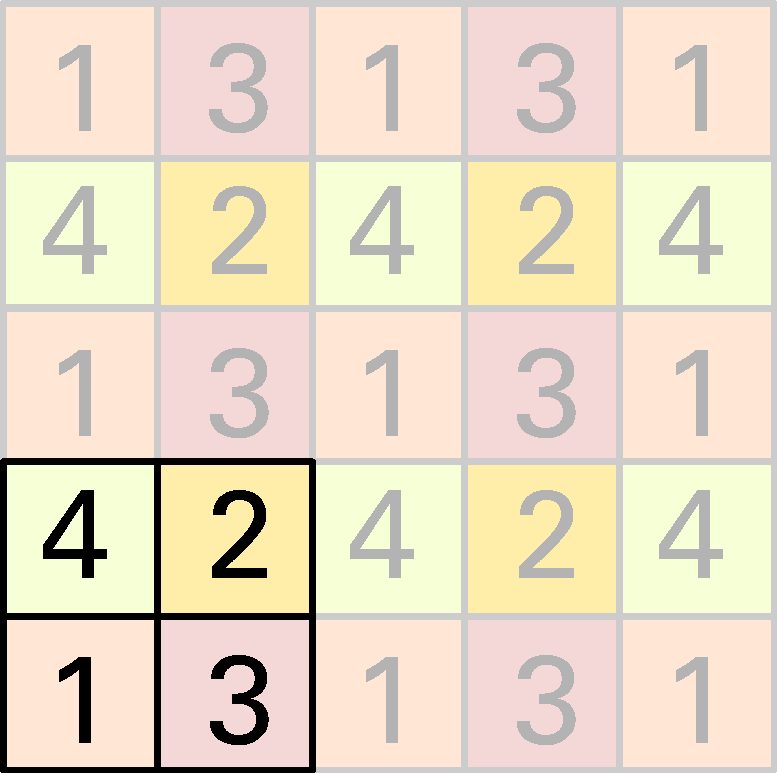
\includegraphics[width=0.4\textwidth]{images/motor_unit_assignment/interleaving_scheme.pdf}%
  \caption{Repeating scheme for interleaving the four partial grids. The partial grids are indicated by the numbers and have different colors. The pattern is highlighted at the bottom left of the figure.}%
  \label{fig:interleaving_scheme}%
\end{figure}

\section{Results and Discussion}\label{sec:mu_results_and_discussion}

In the following, results of the methods described in \cref{sec:method1_assignment,sec:method2_selection,sec:method3_modification} with different parameters are presented.
\Cref{fig:mus_results1} shows the resulting assignment of MUs to fibers for methods 1 and 2. The number of fibers per coordinate direction is $n=13$, a number of $n_\text{MU} = 10$ MUs is considered and two different values for the kernel function parameter $\sigma$ are used.

In \cref{fig:MU_fibre_distribution_13x13_10_2d_fiber_distribution}, method 1 is used with basis $b=1.2$ and a kernel function with standard deviation of a tenth of the grid, $\sigma=n/10$. Each square represents one fiber, their colors refer to the MU index as indicated by the legend. Colored crosses visualize the center points $\bfx_{k_\text{MU}}$ of the respective MUs.

It can be seen that the MU territories, i.e., the regions of the fibers of an MU are located around the center points of the MUs. Because of the random sampling, the fibers of an MU are not all located closely together but spread over a larger area. Especially for MU 8, depicted by light orange color, some fibers are located further away from the center point, which is approximately at the center of the grid. On the other hand, for MU 10 most of the red marked fibers are located close to the center point of the MU, which can be found in the center of the lower third of the grid.

\begin{figure}%
  \centering%
  \begin{subfigure}[t]{0.48\textwidth}%
    \centering%
    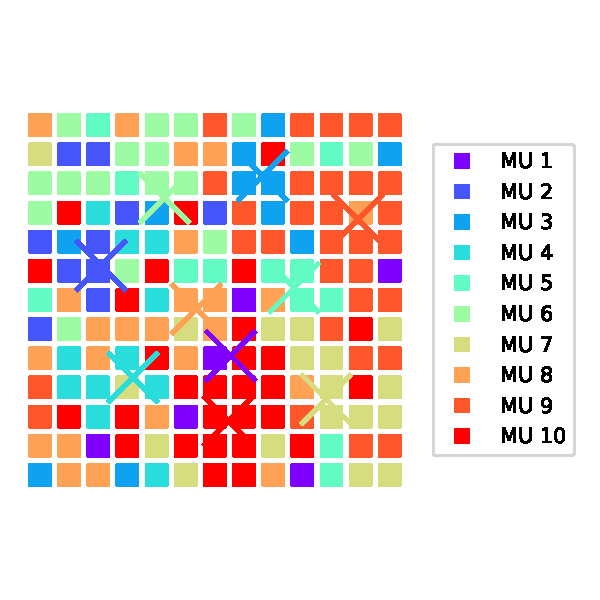
\includegraphics[width=\textwidth]{images/motor_unit_assignment/MU_fibre_distribution_13x13_10_2d_fiber_distribution.pdf}%
    \caption{Result for method 1 with $\sigma = n/10 = 1.3$}%
    \label{fig:MU_fibre_distribution_13x13_10_2d_fiber_distribution}%
  \end{subfigure}
  \quad
  \begin{subfigure}[t]{0.48\textwidth}%
    \centering%
    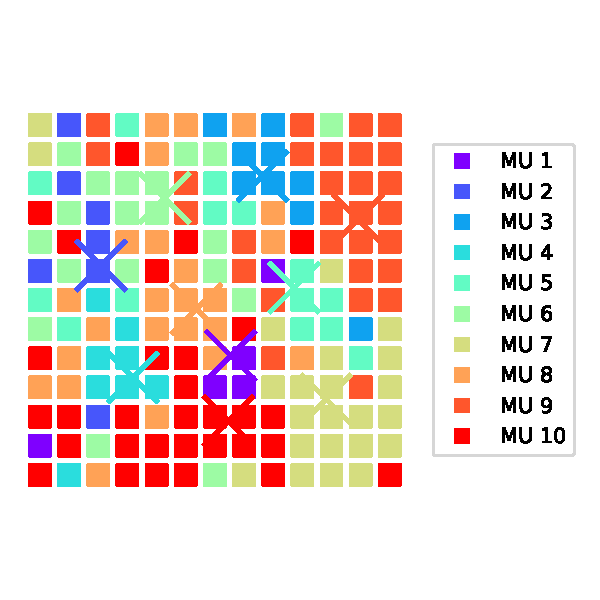
\includegraphics[width=\textwidth]{images/motor_unit_assignment/MU_fibre_distribution_13x13_10_2d_fiber_distribution_sigma.pdf}%
    \caption{Result for method 1 with $\sigma = n/100 = 0.13$}%
    \label{fig:MU_fibre_distribution_13x13_10_2d_fiber_distribution_sigma}%
  \end{subfigure}
  \begin{subfigure}[t]{0.48\textwidth}%
    \centering%
    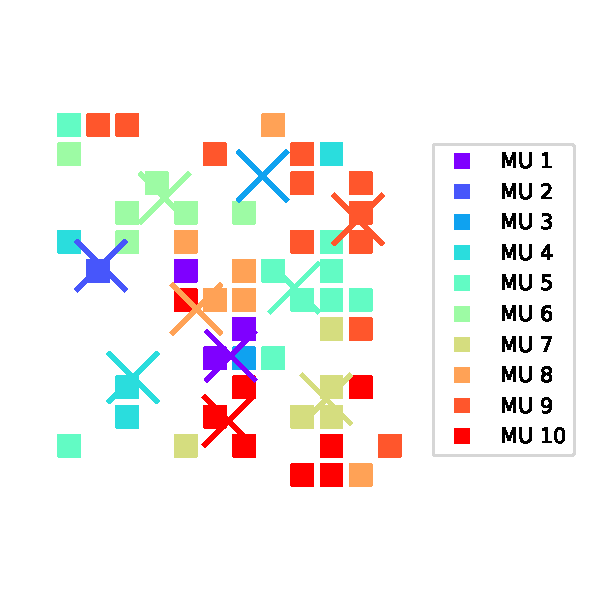
\includegraphics[width=\textwidth]{images/motor_unit_assignment/MU_fibre_distribution_sparse_13x13_10_2d_fiber_distribution.pdf}%
    \caption{Result for method 2 with $\sigma = n/10 = 1.3$, only 54 out of 169 fibers, i.e., \SI{32}{\percent} have an assigned motor unit.}%
    \label{fig:MU_fibre_distribution_sparse_13x13_10_2d_fiber_distribution}%
  \end{subfigure}
  \quad
  \begin{subfigure}[t]{0.48\textwidth}%
    \centering%
    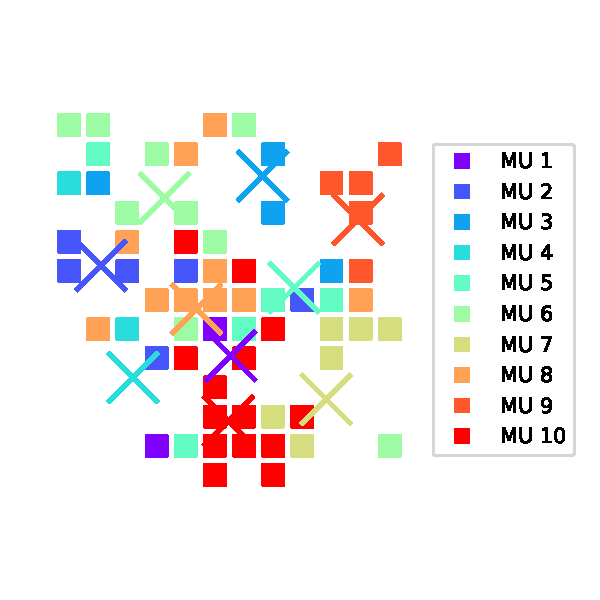
\includegraphics[width=\textwidth]{images/motor_unit_assignment/MU_fibre_distribution_sparse_13x13_10_sigma_2d_fiber_distribution.pdf}%
    \caption{Result for method 2 with $\sigma = n/100 = 0.13$, only 63 out of 169 fibers, i.e., \SI{37}{\percent} have an assigned motor unit.}%
    \label{fig:MU_fibre_distribution_sparse_13x13_10_sigma_2d_fiber_distribution}%
  \end{subfigure}
  \caption{Resulting MU assignments to a grid of $n\times n = 13 \times 13 = 169$ fibers. Each MU is represented by a color, the MU center points $\bfx_{k_\text{MU}}$ are the same for all scenarios and are shown by the colored crosses.}%
  \label{fig:mus_results1}%
\end{figure}%

The histogram for the setting considered in \cref{fig:MU_fibre_distribution_13x13_10_2d_fiber_distribution} is shown in \cref{fig:MU_fibre_distribution_13x13_10_fiber_distribution}. It can be seen that the number of fibers per motor unit approximately follows the prescribed exponential function with basis $b=1.2$. The observed deviation is due to the random sampling.

\begin{figure}%
  \centering%
  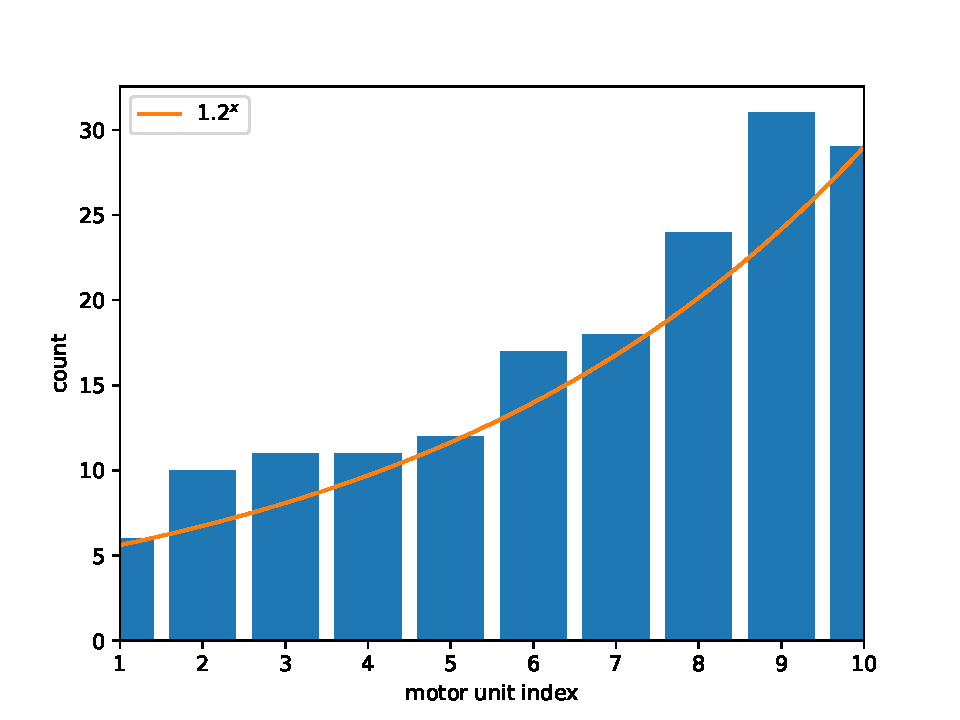
\includegraphics[width=0.8\textwidth]{images/motor_unit_assignment/MU_fibre_distribution_13x13_10_fiber_distribution.pdf}%
  \caption{Histogram of the number of fibers per MU in \cref{fig:MU_fibre_distribution_13x13_10_2d_fiber_distribution}. The orange line corresponds to the ideal exponential distribution $y=c\cdot 1.2^x$.}%
  \label{fig:MU_fibre_distribution_13x13_10_fiber_distribution}%
\end{figure}

\Cref{fig:mu_kernel_fkt} shows the values of the probability function of a specific MU for all fibers, formulated in \cref{eq:mu_p}. \Cref{fig:MU_fibre_distribution_13x13_10_fibers_mu3,fig:MU_fibre_distribution_13x13_10_fibers_mu9} correspond to the scenario considered in \cref{fig:MU_fibre_distribution_13x13_10_2d_fiber_distribution}. The comparison shows that the probability is highest around the center of MU 3 and MU 9, respectively. When moving away from the MU centers, the probability follows approximately the shape of the radial kernel function in \cref{eq:phat_kernel}.
An image of the radial kernel function in higher resolution is given by \cref{fig:MU_fibre_distribution_37x37_50_fibers_mu41}, where the probability function is depicted for MU 41 in a scenario with 50 MUs in a grid of $37 \times 37$ fibers.

It can be observed, however, that the probability distribution in \cref{fig:MU_fibre_distribution_13x13_10_fibers_mu3,fig:MU_fibre_distribution_13x13_10_fibers_mu9} does not entirely follow the kernel function. The effects of the scaling factors $\{\lambda_k\}$ in \cref{eq:mu_p} are visible, e.g., at the top-most and right-most fibers. There, the probability increases again compared to the interior of the grid. The purpose of the scaling factors is to enforce the exponential distribution of MU sizes.

\begin{figure}%
  \centering%
  \begin{subfigure}[t]{0.31\textwidth}%
    \centering%
    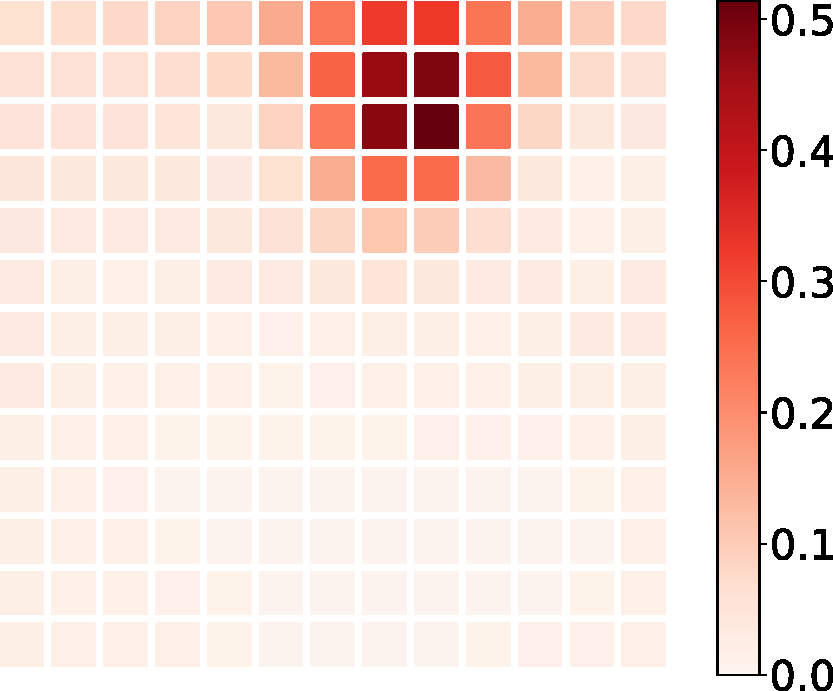
\includegraphics[width=\textwidth]{images/motor_unit_assignment/MU_fibre_distribution_13x13_10_fibers_mu3.pdf}%
    \caption{$n=13, \sigma = n/10 = 0.13$, MU 3}%
    \label{fig:MU_fibre_distribution_13x13_10_fibers_mu3}%
  \end{subfigure}
  \quad
  \begin{subfigure}[t]{0.31\textwidth}%
    \centering%
    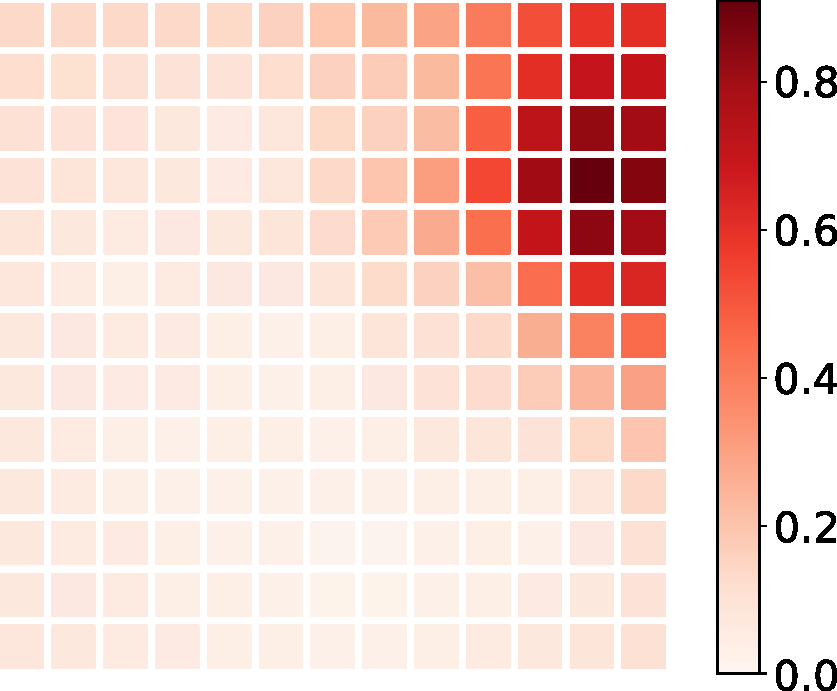
\includegraphics[width=\textwidth]{images/motor_unit_assignment/MU_fibre_distribution_13x13_10_fibers_mu9.pdf}%
    \caption{$n=13, \sigma = n/10 = 0.13$, MU 9}%
    \label{fig:MU_fibre_distribution_13x13_10_fibers_mu9}%
  \end{subfigure}
  \quad
  \begin{subfigure}[t]{0.31\textwidth}%
    \centering%
    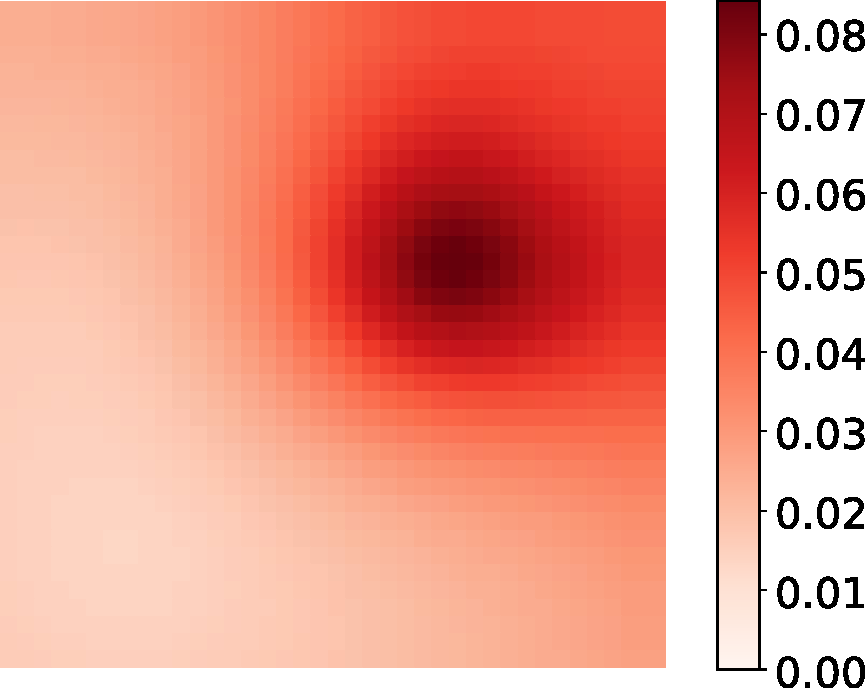
\includegraphics[width=\textwidth]{images/motor_unit_assignment/MU_fibre_distribution_37x37_50_fibers_mu41.pdf}%
    \caption{$n=37, \sigma = n/10 = 0.37$, MU 41}%
    \label{fig:MU_fibre_distribution_37x37_50_fibers_mu41}%
  \end{subfigure}
  \caption{Probability at every fiber to be in a given MU, for different grid sizes and number of MUs.}%
  \label{fig:mu_kernel_fkt}%
\end{figure}%

This effect is illustrated more clearly in \cref{fig:MU_fibre_distribution_13x13_10_pdf}. It shows the value of $p(i,j,k_\text{MU})$ for the top right fiber in the grid, $(i,j)=(13,13)$, for all values of $k_\text{MU}$. The blue curve indicates the probability that results from the kernel functions, only according to the distance of the top right fiber to the respective MU centers. In other words, the scaling factors $\{\lambda_k\}_{1\dots n_\text{MU}}$ are removed or equivalently set to one. By inspecting again \cref{fig:MU_fibre_distribution_13x13_10_2d_fiber_distribution}, it can be seen that the MU centers of MUs 9, 3 and 5 are---in this order---closest to the top right fiber whereas MU 4 and 10 are the furthest away. Consequently, the blue curve in \cref{fig:MU_fibre_distribution_13x13_10_pdf} has peaks at 9, 3 and 5 and low values for 4 and 10.

When incorporating the scaling factors $\{\lambda_k\}_{1\dots n_\text{MU}}$ that were found by the optimization problem in \cref{eq:mus_opt}, the probabilities change to the orange curve. It can be seen that the probability for the fiber to be in MU 9 increases. MU 9 which is expected to have a rather high number of fibers according to the exponential progression.
It gets more fibers from the top right corner. The areas left to and below the center of MU 9 are at the same time close to the centers of MU 3 and 5 and therefore can also be occupied by fibers of MUs 3 and 5. Thus, the optimization performs an exchange where MU 9 forgoes the bottom and left fibers and, conversely, obtains portions of the fibers in the top right area from MUs 3 and 5. Consequently, the probability in \cref{fig:MU_fibre_distribution_13x13_10_pdf} decreases for MUs 3 and 5. The shape of the final probability distribution for MU 9 in \cref{fig:MU_fibre_distribution_13x13_10_fibers_mu9} is the kernel function stretched to the top and right.
By looking at \cref{fig:MU_fibre_distribution_13x13_10_2d_fiber_distribution}, it can be seen that, by chance, the top right fiber indeed gets assigned to MU 9.

\begin{figure}%
  \centering%
  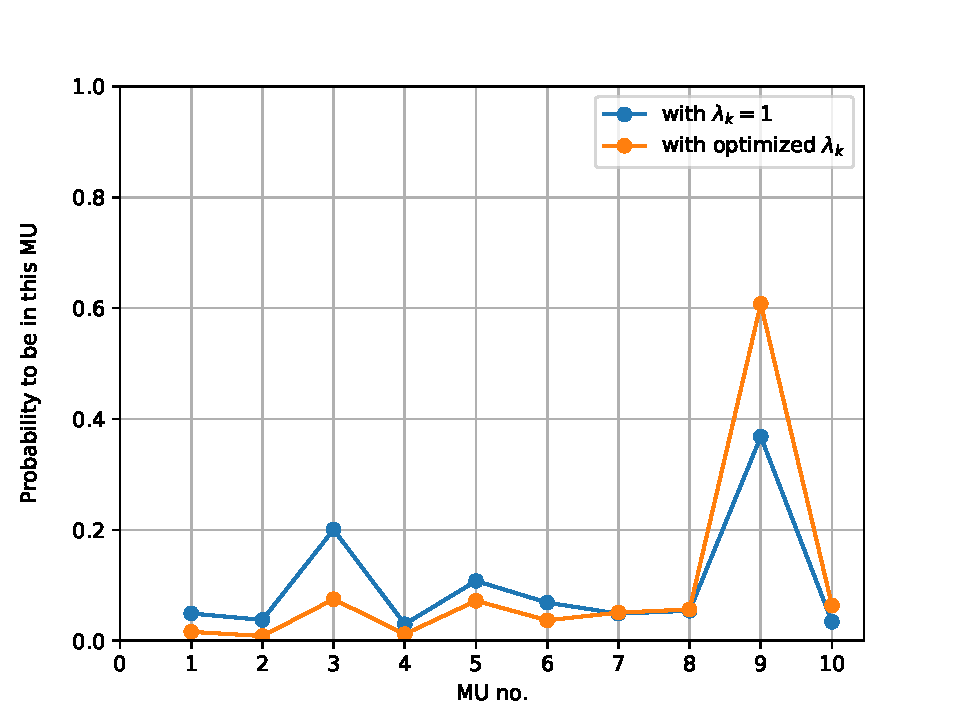
\includegraphics[width=0.8\textwidth]{images/motor_unit_assignment/MU_fibre_distribution_13x13_10_pdf.pdf}%
  \caption{Probability of the top right fiber in the $13 \times 13$ grid to be in a given MU, without considering the scaling factors $\{\lambda_k\}_{1\dots n_\text{MU}}$ (blue) and including the scaling factors (orange).}%
  \label{fig:MU_fibre_distribution_13x13_10_pdf}%
\end{figure}

The influence of the kernel width $\sigma$ is demonstrated by comparing \cref{fig:MU_fibre_distribution_13x13_10_2d_fiber_distribution} with \cref{fig:MU_fibre_distribution_13x13_10_2d_fiber_distribution_sigma}. In \cref{fig:MU_fibre_distribution_13x13_10_2d_fiber_distribution_sigma} the value of $\sigma$ is only a tenth of the value in \cref{fig:MU_fibre_distribution_13x13_10_2d_fiber_distribution}. All other parameters are the same such that a similar exponential distribution of MU sizes is obtained. It can be seen that the MU territories are less interleaved and have clearer borders. For example, the territory of MU 7 at the bottom left of the domain has a cohesive shape in \cref{fig:MU_fibre_distribution_13x13_10_2d_fiber_distribution_sigma} whereas the respective fibers are more scattered in \cref{fig:MU_fibre_distribution_13x13_10_2d_fiber_distribution}.

In comparison, the results for method 2 with the same two values of $\sigma$ are shown in \cref{fig:MU_fibre_distribution_sparse_13x13_10_2d_fiber_distribution,fig:MU_fibre_distribution_sparse_13x13_10_sigma_2d_fiber_distribution}. All other parameters are kept the same. It can be seen how method 2 only associates some fibers with MUs. For the larger standard deviation $\sigma$ in \cref{fig:MU_fibre_distribution_sparse_13x13_10_2d_fiber_distribution}, only \SI{32}{\percent} of the fibers get assigned to a MU, for the smaller value of $\sigma$, the fraction is slightly higher with \SI{37}{\percent}. Similar to method 1, the effect of more cohesive MU territories for smaller $\sigma$ values can also be observed in the results of method 2.

Next, the two methods 1 and 2 are investigated for a higher number of $n_\text{MU}=100$ motor units and a grid of $n \times n=67 \times 67 = \num{4489}$ fibers.

\Cref{fig:MU_fibre_distribution_67x67_100_mu_positions} shows the MU center points $\bfx_{k_\text{MU}}$. The color corresponds to the MU index and follows the same rainbow color scheme as in \cref{fig:mus_results1}. Since the construction scheme is the deterministic Weyl sequence in \cref{eq:weyl}, the first 10 MU center positions are the same as for the scenario with $n_\text{MU}=10$. It can be seen that the MU centers have similar distances throughout the grid and that, in general, MUs located next to each other have different colors and therefore are differently sized.

\Cref{fig:MU_fibre_distribution_67x67_100_fiber_distribution} shows the histogram of the MUs, i.e., the number of fibers per MU. Following \cite{Enoka2001} the prescribed basis for the exponential progression was reduced because of the higher number of fibers. It was set to $b=1.05$. It can be seen that the resulting MU size distribution closely matches the prescribed function. Because the ratio of fibers to MUs (4489/100) is higher than in the previous setting (169/10) the deviation of the realized MU sizes from the prescribed curve appears smaller than in \cref{fig:MU_fibre_distribution_13x13_10_fiber_distribution}.

\Cref{fig:MU_fibre_distribution_67x67_100_some_2d_fiber_distribution.pdf} shows the result for method 1. The width of the radial kernel function was chosen as $\sigma = n/100 = \num{0.67}$. Only the fibers of five selected MUs and their center points are visualized for better clearity.

The algorithm for the 4489 fibers and 100 MUs was performed with a  chunk size of $n_\text{per\_chunk}=10$, yielding a total number of $n_\text{chunks}=10$ chunks. The runtime was \SI{45}{\min} \SI{53.5}{\sec} on a single core of an Intel Core i5-6300U CPU with base frequency of 2.40GHz and 19.5 GiB of RAM.

\Cref{fig:MU_fibre_distribution_sparse2_67x67_100_2d_fiber_distribution} shows the result for method 2. All resulting fibers that were associated to an MU are shown as gray or colored squares, leaving white spaces for unassigned fibers. Again, only the fibers of five selected MUs are colored. The kernel parameter was set to $\sigma = 0.04\cdot n = \num{2.68}$ which resulted in 2328 of 4489 fibers or \SI{52}{\percent} of the fibers being assigned an MU. When the parameter is instead set to $\sigma = n/100  = \num{0.67}$ as in the study with 10 MUs before, the result assigns only 136 fibers or \SI{3}{\percent}. This shows that method 2 is very sensitive to the choice of the standard deviation parameter $\sigma$.

The comparison with \cref{fig:MU_fibre_distribution_67x67_100_some_2d_fiber_distribution.pdf} shows that the resulting MU territories are more dispersed than for method 1. This can be explained with the higher value of $\sigma$. Obtaining \say{sharper} MU territories would require a smaller $\sigma$, however, this results in less fibers being assigned to MUs.

Furthermore, \cref{fig:MU_fibre_distribution_sparse2_67x67_100_2d_fiber_distribution} shows that the fiber density decreases towards the outer border of the domain. In reality, staining studies on skeletal muscles do not find this effect.
%In an electrophysiology simulation with muscle fibers where the aim is to compute EMG signals on the surface of a muscle, this effect is not desired, as the border of the domain is the important part that contributes to the measurements of surface EMG.

An advantage of method 2 over method 1 is that we do not have to solve any optimization problem. In consequence, the algorithm for the scenario in \Cref{fig:MU_fibre_distribution_sparse2_67x67_100_2d_fiber_distribution} was completed in \SI{8}{\sec} on the same hardware as before.

\begin{figure}%
  \centering%
  \begin{subfigure}[t]{0.48\textwidth}%
    \centering%
    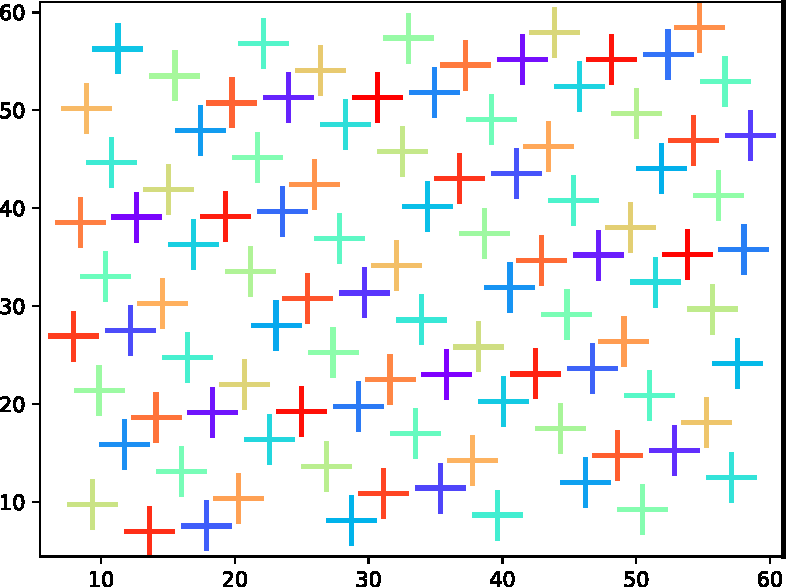
\includegraphics[width=\textwidth]{images/motor_unit_assignment/MU_fibre_distribution_67x67_100_mu_positions.pdf}%
    \caption{MU center points.}%
    \label{fig:MU_fibre_distribution_67x67_100_mu_positions}%
  \end{subfigure}
  \quad
  \begin{subfigure}[t]{0.48\textwidth}%
    \centering%
    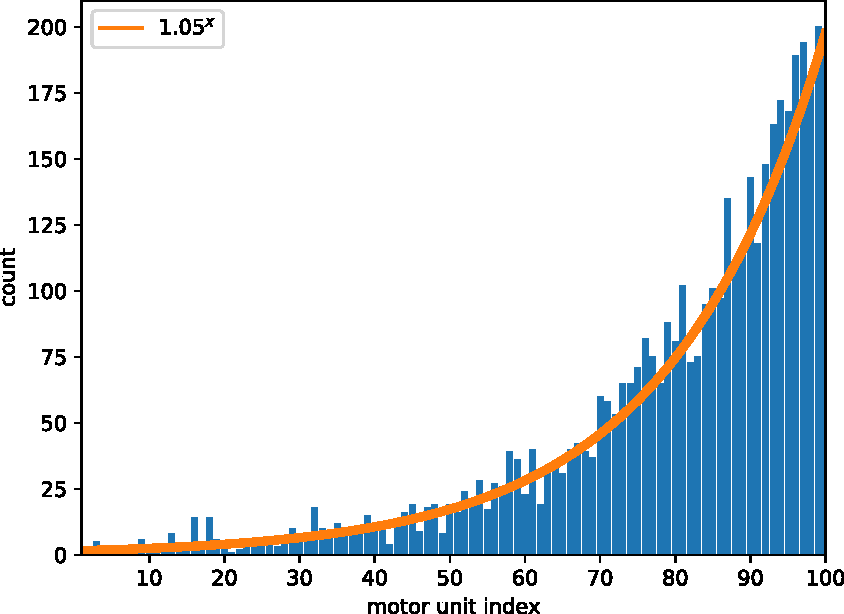
\includegraphics[width=\textwidth]{images/motor_unit_assignment/MU_fibre_distribution_67x67_100_fiber_distribution.pdf}%
    \caption{Histogram of number of fibers assigned to MUs (blue) and the prescribed exponential progression $y=c\cdot 1.05^x$ (orange).}%
    \label{fig:MU_fibre_distribution_67x67_100_fiber_distribution}%
    %total number of fibers: 4489
  %  MU 11, n. fibers optimal: 2.802, n. fibers expected: 0.945, realized: 1
  %MU 41, n. fibers optimal: 12.108, n. fibers expected: 8.809, realized: 15
  %MU 61, n. fibers optimal: 32.126, n. fibers expected: 30.439, realized: 29
  % MU 81, n. fibers optimal: 85.241, n. fibers expected: 127.908, realized: 118
  %MU 91, n. fibers optimal: 138.849, n. fibers expected: 137.036, realized: 123
  
  \end{subfigure}
  \begin{subfigure}[t]{0.48\textwidth}%
    \centering%
    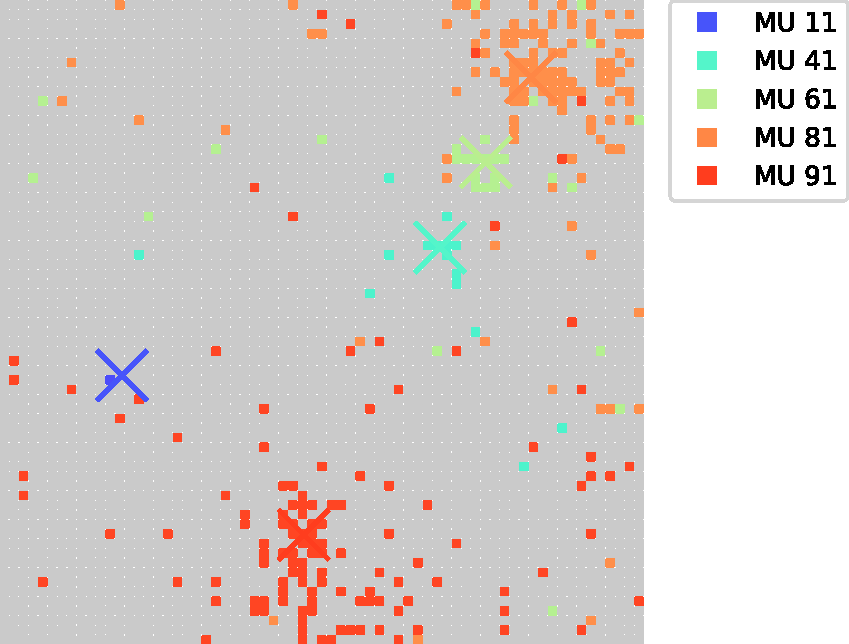
\includegraphics[width=\textwidth]{images/motor_unit_assignment/MU_fibre_distribution_67x67_100_some_2d_fiber_distribution.pdf}%
    \caption{Result of method 1 with $\sigma = n/100 = \num{0.67}$. The colored fibers are assigned to one of five selected MUs: 11, 41, 61, 81 and 91. The MU sizes are: 
    MU 11: 1 fiber,
    MU 41: 2 fibers,
    MU 61: 15 fibers,
    MU 81: 32 fibers,
    MU 91: 72 fibers}%
    \label{fig:MU_fibre_distribution_67x67_100_some_2d_fiber_distribution.pdf}%
  \end{subfigure}
  \quad
  \begin{subfigure}[t]{0.48\textwidth}%
    \centering%
    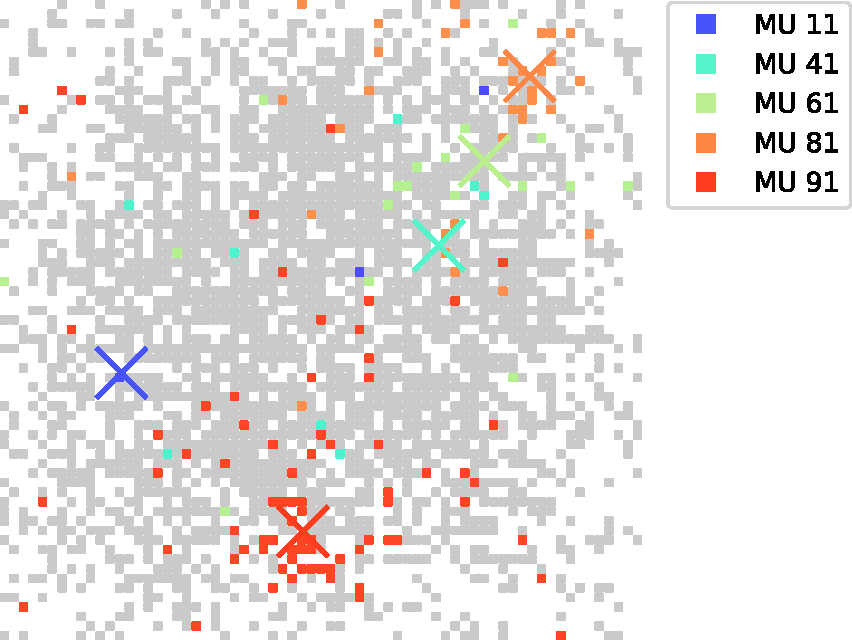
\includegraphics[width=\textwidth]{images/motor_unit_assignment/MU_fibre_distribution_sparse2_67x67_100_2d_fiber_distribution.pdf}%
    \caption{Result of method 2 with $\sigma = 0.04\cdot n = \num{2.68}$. The colored fibers are assigned to one of five selected MUs: 11, 41, 61, 81 and 91. The MU sizes are:  
    MU 11: 3 fibers, MU 41: 8 fibers, MU 61: 18 fibers, MU 81: 34 fibers, MU 91: 75 fibers}%
    \label{fig:MU_fibre_distribution_sparse2_67x67_100_2d_fiber_distribution}%
  \end{subfigure}
  \caption{Results of the presented algorithm to assign MUs to fibers, using a grid of $67 \times 67$ fibers and 100 MUs.}%
  \label{fig:100mus_results}%
\end{figure}%

%chunksize 10, Total duration: 352.44 s 
% MU_fibre_distribution_combined_67x67_100.txt_2d_fiber_distribution_.pdf
% MU_fibre_distribution_combined_67x67_100.txt_fiber_distribution_.pdf
% MU_fibre_distribution_combined_67x67_100_0_2d_fiber_distribution_.pdf
% MU_fibre_distribution_combined_67x67_100_1.txt_2d_fiber_distribution_.pdf
% MU_fibre_distribution_combined_67x67_100_2.txt_2d_fiber_distribution_.pdf
% MU_fibre_distribution_combined_67x67_100_3.txt_2d_fiber_distribution_.pdf

%chunksize 5, Total duration: 293.03 s

% sparse:
% MU_fibre_distribution_combined_sparse_251x251_100_2d_fiber_distribution.pdf

Next, the extension of methods 1 and 2, called 1a and 2a, are investigated that ensure that neighboring fibers are not associated to the same MU.
\Cref{fig:mu_method3_partial} shows results for method 1a for $n_\text{MU}=100$ MUs. In \cref{fig:mu_3partial_1,fig:mu_3partial_2,fig:mu_3partial_3}, three of the four partial grids with $n=34$ are shown. 
Because parameters are the same for those smaller grids, the generated MU assignments look similar for all partial grids, except for different MU center positions. In \cref{fig:mu_3_1}, the resulting grid with $n=67$ is shown that is obtained by interleaving the four partial grids. In this MU association, all neighboring fibers belong to different MUs. The resulting distribution of MU sizes is shown in \cref{fig:mu_method3_distribution}. It can be seen that the algorithm for method 1a achieves the approximate, prescribed exponential progression.

An advantage of method 1a is also that the runtime decreases compared to method 1. The result in \cref{fig:mu_3_1} could be computed in \SI{5}{\min} \SI{52.4}{\sec} with $n_\text{per\_chunk}=10$ or in \SI{4}{\min} \SI{53.0}{\sec} with $n_\text{per\_chunk}=5$, compared to the \SI{45}{\min} \SI{53.5}{\sec} of method 1.

\begin{figure}%
  \centering%
  \begin{subfigure}[t]{0.48\textwidth}%
    \centering%
    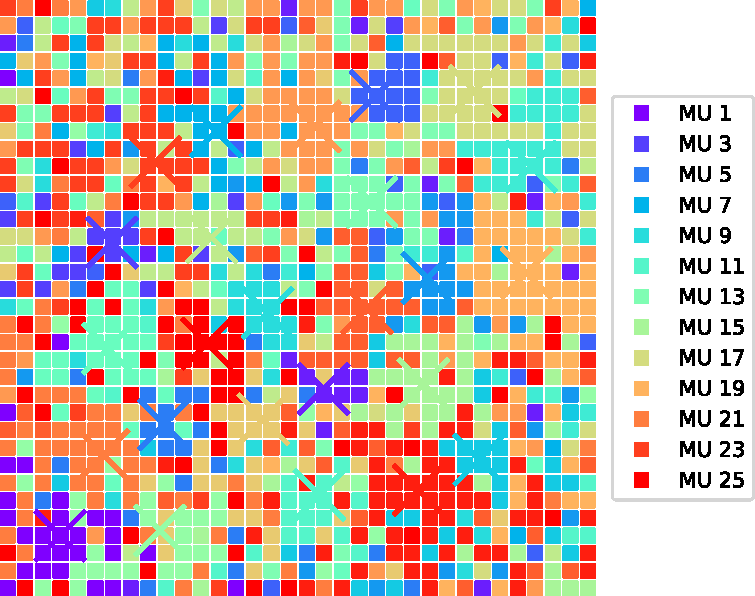
\includegraphics[width=\textwidth]{images/motor_unit_assignment/MU_fibre_distribution_combined_67x67_100_0_2d_fiber_distribution_.pdf}%
    \caption{First partial grid, $n=34$.}%
    \label{fig:mu_3partial_1}%
  \end{subfigure}
  \,
  \begin{subfigure}[t]{0.48\textwidth}%
    \centering%
    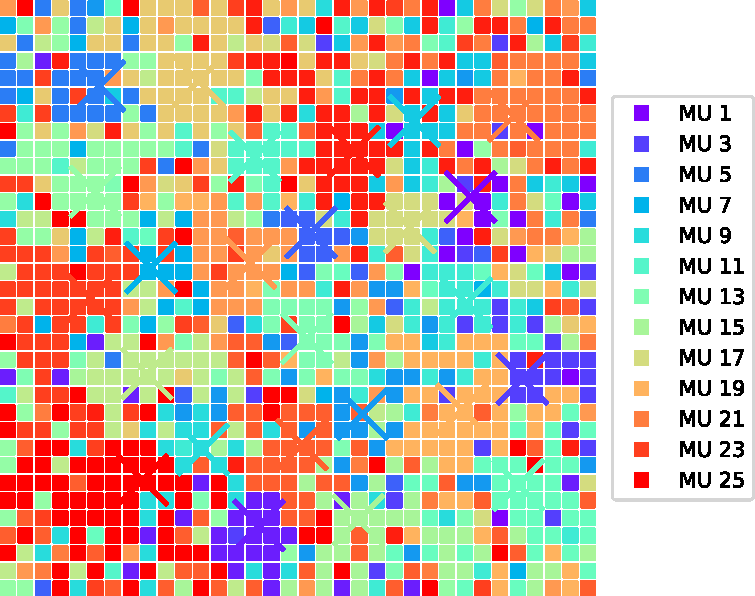
\includegraphics[width=\textwidth]{images/motor_unit_assignment/MU_fibre_distribution_combined_67x67_100_1_2d_fiber_distribution_.pdf}%
    \caption{Second partial grid, $n=34$.}%
    \label{fig:mu_3partial_2}%
  \end{subfigure}
  \,
  \begin{subfigure}[t]{0.48\textwidth}%
    \centering%
    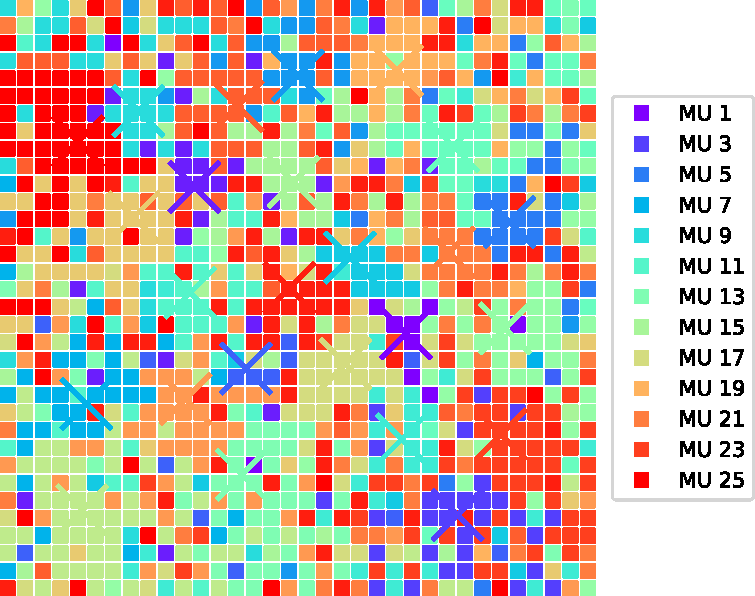
\includegraphics[width=\textwidth]{images/motor_unit_assignment/MU_fibre_distribution_combined_67x67_100_2_2d_fiber_distribution_.pdf}%
    \caption{Third partial grid, $n=34$.}%
    \label{fig:mu_3partial_3}%
  \end{subfigure}
  \,
%  \begin{subfigure}[t]{0.48\textwidth}%
%    \centering%
%    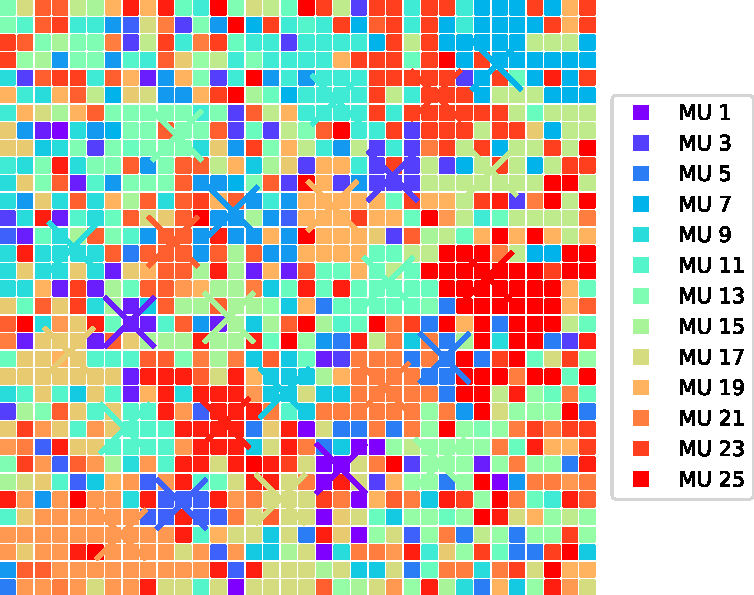
\includegraphics[width=\textwidth]{images/motor_unit_assignment/MU_fibre_distribution_combined_67x67_100_3_2d_fiber_distribution_.pdf}%
%    \caption{Forth partial grid.}%
%    \label{fig:mu_3partial_4}%
%  \end{subfigure}
  \begin{subfigure}[t]{0.48\textwidth}%
    \centering%
    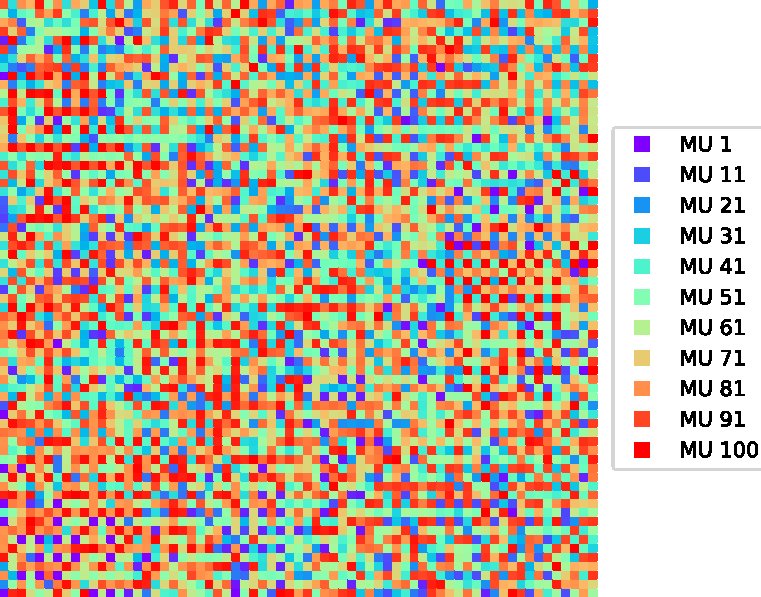
\includegraphics[width=\textwidth]{images/motor_unit_assignment/MU_fibre_distribution_combined_67x67_100_2d_fiber_distribution_.pdf}%
    \caption{Resulting interleaved grid, $n=67$.}%
    \label{fig:mu_3_1}%
  \end{subfigure}
  \caption{Assignment of motor units to fibers using method 1a. Shown are the first three partial grids (a)-(c) to be interleaved and the result (d), parameters $n=67, n_\text{MU}=100, \sigma = n/10 = 6.7, b=1.05$}%
  \label{fig:mu_method3_partial}%
\end{figure}%


\begin{figure}%
  \centering
  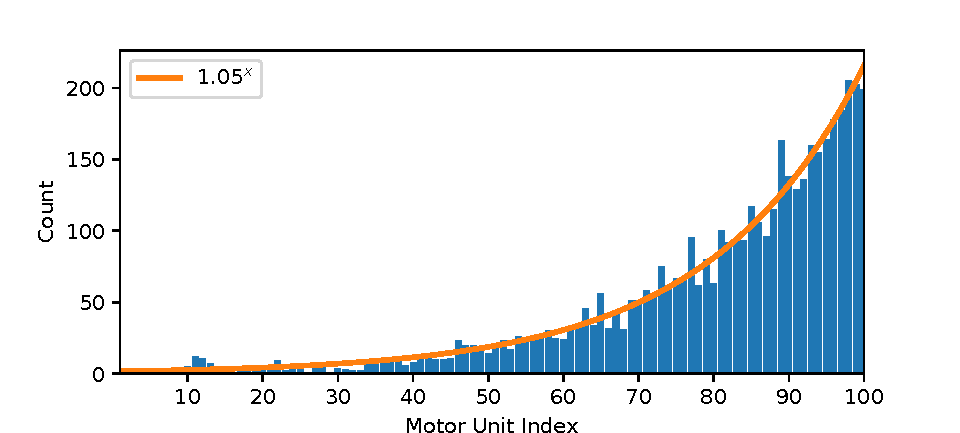
\includegraphics[width=0.9\textwidth]{images/motor_unit_assignment/MU_fibre_distribution_combined_67x67_100_fiber_distribution.pdf}%
  \caption{Histogram of number of fibers assigned to MUs for method 1a, for the scenario that is shown in \cref{fig:mu_method3_partial}.}%
  \label{fig:mu_method3_distribution}%
\end{figure}%

Method 2a cannot be reasonably used with the same parameters as method 1a. If it is used to generate fibers assigned to 100 MUs, a grid of $67 \times 67$ leads to the majority of MUs having only 1 fiber. Therefore, a larger grid is needed. \Cref{fig:mu_method3_2} shows the result for $n=251$. The result assigns \num{13618} of the $n^2 = \num{63001}$ initial fibers to MUs, i.e. \SI{22}{\percent}. The number of fibers per MU varies between \num{41} and \num{244}. As can be seen, fibers of the same MU are separated by either a fiber of a different MU or by a an unassigned fiber, i.e., a hole in the grid.

%It can be seen in \cref{fig:mu_method3_2} that the fibers are dispersed over the grid and holes are present throughout the domain. The resulting set of fibers can be viewed as being arbitrarily positioned in the domain instead of following the grid. When this viewpoint is adopted, the property that neighboring fibers are of different MUs no longer holds as the separation is often given by a hole, which does not prevent the fibers touching each other.

\begin{figure}%
  \centering
  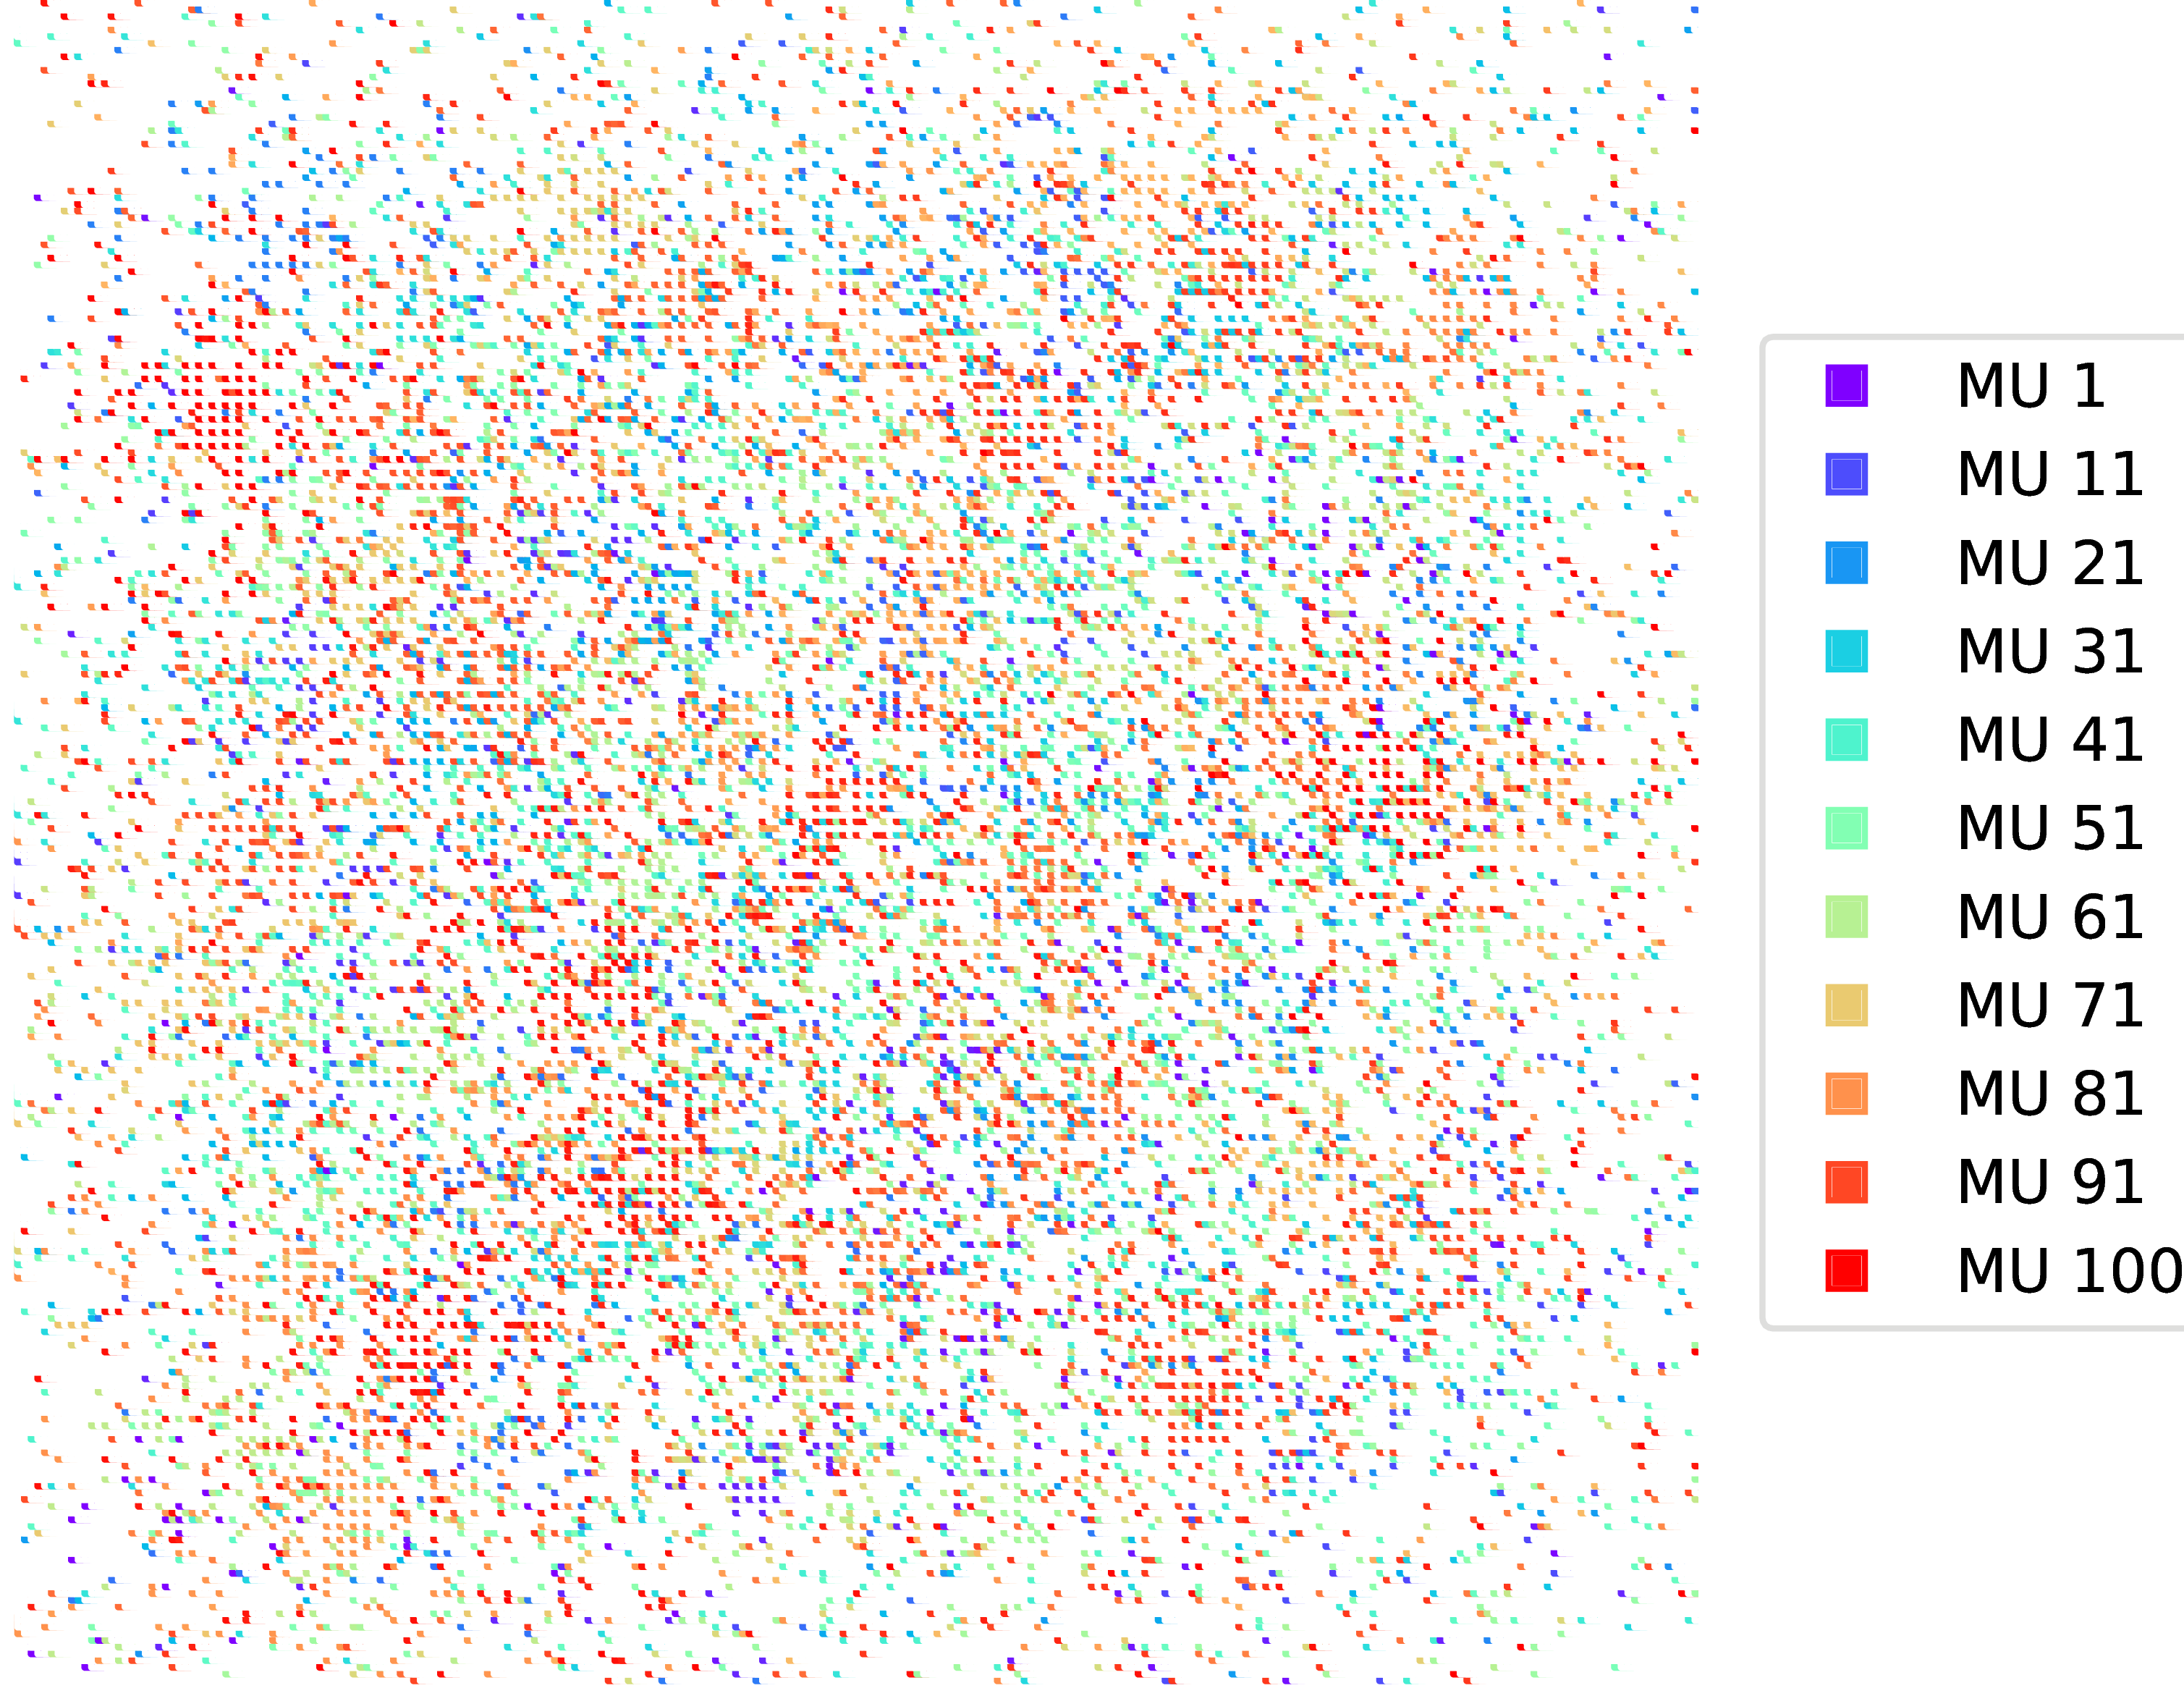
\includegraphics[width=0.9\textwidth]{images/motor_unit_assignment/MU_fibre_distribution_combined_sparse_251x251_100_2d_fiber_distribution_.png}%
  \caption{Assignment of motor units to fibers using method 2a and parameters $n=251, n_\text{MU}=100, \sigma = n/100 = 2.51, b=1.05$.}%
  \label{fig:mu_method3_2}%
\end{figure}%
% resulting fibers: 13618 / 63001 = 22\%

\begin{reproduce}
  Run the script \code{generate_fiber_distribution.py} without arguments to get usage information.
  The script contains the implementation for all three presented methods. For example, to run method 1a to get the result of \cref{fig:mu_method3_partial}, use:
  \begin{lstlisting}[columns=fullflexible,breaklines=true,postbreak=\mbox{\textcolor{gray}{$\hookrightarrow$}\space}]
    generate_fiber_distribution.py MU_fibre_distribution_combined_67x67_100 100 3 1 67 1.05 100 10
  \end{lstlisting}
  Then, existing fiber distribution files can be visualized by the following script:
  \begin{lstlisting}[columns=fullflexible,breaklines=true,postbreak=\mbox{\textcolor{gray}{$\hookrightarrow$}\space}]
    $\$$OPENDIHU_HOME/examples/electrophysiology/input/plot_fibre_distribution_2d.py MU_fibre_distribution_combined_67x67_100.txt 67
  \end{lstlisting}
\end{reproduce}

\section{Summary and Conclusion}\label{sec:mu_conclusion}
In the beginning of this chapter, two methods 1 and 2 for associating MUs with fibers in a given 2D grid were presented. The methods were constructed based on biophysical properties of MU distribution. The fibers were located in intermingling MU territories that were each centered at different MU center points.
The density of fibers belonging to an MU decreased with higher distance from the center and was described by a radial kernel function.
The number of fibers assigned to the motor units approximately followed an exponential progression where the first MU contained the lowest number of fibers and the last MU contained the largest amount. 
Whereas method 1 assigned MUs to all available fibers, method 2 only assigned MUs to some fibers yielding a lower number of fibers in the result.
Evaluation of the literature showed that no comparable method with these properties existed previously.

Next, the methods 1a and 2a were introduced that built upon methods 1 and 2. They ensured that neighboring fibers were assigned to different MUs, another behavior that was known from anatomical studies.

Steps of the algorithms and their final satisfaction of the design critera were demonstrated with various visualizations. Results were shown for different parameter values. The influence of the kernel width on the \say{sharpness} or intermingledness of MU territories was pointed out. 

It was found that methods 2 and 2a typically produced results where only 20-50\% of the fibers get an MU assigned. This ratio highly depended on the problem size and the kernel function width and no direct predictions about the number of resulting fibers was possible. Since the kernel parameter at the same time also influenced the sharpness of the MU territories, adjusting parameters to the desired outcome was an issue for these methods. Reasonable results were only achieved for a higher number of initial fibers. In contrast, methods 1 and 1a robustly produced exponentially distributed MU assignments for all parameter values.

In method 2a for large grid sizes the fibers were dispersed over the grid and \say{holes}, i.e., unassigned fibers, were present throughout the domain. The fiber density decreased towards the boundaries of the domain. No experimental evidence exists that this behaviour occurs in reality. It might also be unfavorable when EMG simulations are performed where the boundary layers contribute most to the measured EMG signal on the muscle surface. In contrary, method 1a did not show this behavior.

The runtime for \num{4489} fibers and 100 MUs was over \SI{45}{\min} for method 1 and below \SI{10}{\sec} for method 2. The large difference could be explained with the optimization problem that needed to be solved for method 1. To handle large runtimes for a high number of MUs, an algorithm was presented that splits the optimization problem in smaller chunks that could be solved faster.

With the use of the extended methods 1a and 1b, runtime decreased. For method 1a the runtime was under \SI{6}{\min}. These runtimes are all considered acceptable since the task occurs only once during preprocessing. 

In conclusion, the developed method 1a proved to be robust for all tested parameter combinations and fulfilled all considered biophysical properties of MU distributions. The exponential distribution of MU sizes and the sharpness of MU territories are adjustable through parameters. If the condition that neighboring fibers belong to different MUs is not desired, method 1 can be used instead.

The presented methods are implemented and made available as Open Source software within \opendihu{}.
The program stores the resulting MU assignments in a plain text file format that is compatible with both OpenCMISS Iron and \opendihu{}. Thus, it can and will be used in simulations of the multi-scale chemo-electromechanical model.
